\chapter{Développement d'outils d'investigation}
\label{chap:2}
\section{Méthode de modélisation au niveau système}

% Need to simulate from source to input for soft-failure analysis
Une méthodologie de construction de modèles ESD au niveau système est proposée.
Elle permet une simulation précise jusqu'à l'entrée d'un circuit intégré en fonctionnement.
Un environement de test ESD est composé d'éléments récurrents tels que des sources DC, des oscilloscopes, et des générators stress, interconnectés par des cables et des fils.
Les cartes électroniques embarquent différents types de composants, tels que des passifs, des protections ESD, des chokes.
L'objectif de la méthode proposée est de construire une librairie des éléments les plus courants, puis d'assembler le modèle complet du système avec.

% Cables and delays identified as important for esd sims - because of similar order of magnitude
Les cables sont des éléments importants mais parfois négligés dans les simulations ESD.
Ils introduisent des délais de propagation non négligeables par rapport à la durée d'un ESD.
Pour ordre de grandeur, un cable coaxial 50\textOmega{} possède une constante de propagation d'environ 5 ns/m.
En comparaison, un ESD dure entre une dizaine et plusieurs centaines de nanosecondes, ce qui est globablement proche du même ordre de grandeur.
Les câbles sont avant tout des lignes de transmission, dont l'analyse théorique fut faite par J. Maxwell, L. Kelvin et O. Heavyside et énormément étudiées par la suite dans la littérature \cite{branin-tl-ref, hf-coax,lossy-tl,emc-analysis-tl}.

% Distributed model
Dans le domaine de ESD, le modèle le plus populaire de ligne est basé sur des éléments distribués.
Concrètement, c'est une suite réseaux L-C tels que la Fig. \ref{fig:dis-line-model}.
Les valeurs de chaque élément sont calculées à partir des propriétés du cable et de la précision requise pour la simulation.

\begin{figure}[!h]
  \centering
  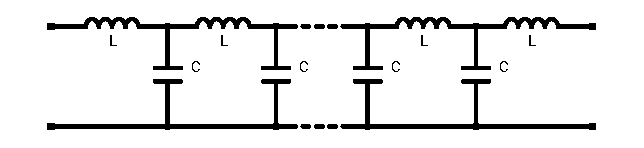
\includegraphics[width=0.7\textwidth]{src/2/figures/lc_ladder.pdf}
  \caption{Electrical distributed LC ladder model of a lossless transmission line}
  \label{fig:dis-line-model}
\end{figure}

% Perks and disavantages
Malgré sa très large adoption, ce modèle présente de sérieux inconvénients.
En particulier, ce modèle nécessite un très grand nombre d'éléments pour avoir une précision décente.
Pour une même précision, le nombre d'éléments est proportionnel à la longueur du cable, ce qui augmente considérablement les temps de simulation.
Pour augmenter la bande passante du modèle, le nombre d'éléments doit également être augmenté.
La combinaison des deux résulte en des temps de simulation très longs.

% Behavioral model
Le modèle à deux ports décrit par H. Branin \cite{branin-tl-ref} est une alternative bien plus sérieuse au modèle distribué.
Il décrit très efficacement et avec une très grande précision le comportement d'une ligne de transmission.
La bande passante n'est pas limité, et le temps de simulation est indépendant de la longueur du câble.
Le modèle est constitué de deux sources de tension controllées en tension et deux résistances (Fig. \ref{fig:beh-line-model}).

\begin{figure}[!h]
  \centering
  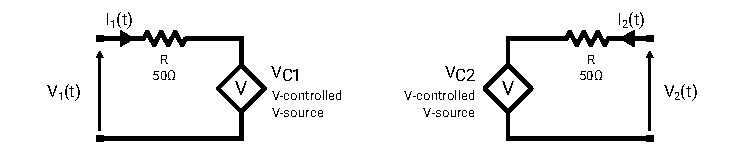
\includegraphics[width=\textwidth]{src/2/figures/behavioral_line_model.pdf}
  \caption{Electrical behavioral model of a lossless transmission line}
  \label{fig:beh-line-model}
\end{figure}

Le comportement des sources est décrit par les équations \ref{eq:beh-line-1} et \ref{eq:beh-line-2}.

\begin{equation}
V_{C1}(t) = V_{2}(t - \Delta t) + Z_{C}.I_{2}(t - \Delta t)
\label{eq:beh-line-1}
\end{equation}

\begin{equation}
V_{C2}(t) = V_{1}(t - \Delta t) + Z_{C}.I_{1}(t - \Delta t)
\label{eq:beh-line-2}
\end{equation}

% Explain the equations
Z\textsubscript{C} est l'impédance charactéristique de la ligne et \textDelta{}t le délai de propagation.
Les équations décrivent un système où tension et courant à chaque port sont la superposition d'une onde se propageant dans un sens et d'une seconde dans l'autre sens.

% Compare both models to know which one is preferrable
Des simulations permettent de comparer les deux modèles.
Une impulsion rectangulaire est injectée sur chaque modèle avec un temps de montée de 1ps.
Différentes charges permettent d'évaluer les performances et la précision.
Les lignes de transmission ont un délai de 100ns et une impédance charactéristique de 50\textOmega{}.

\begin{figure}[!h]
  \centering
  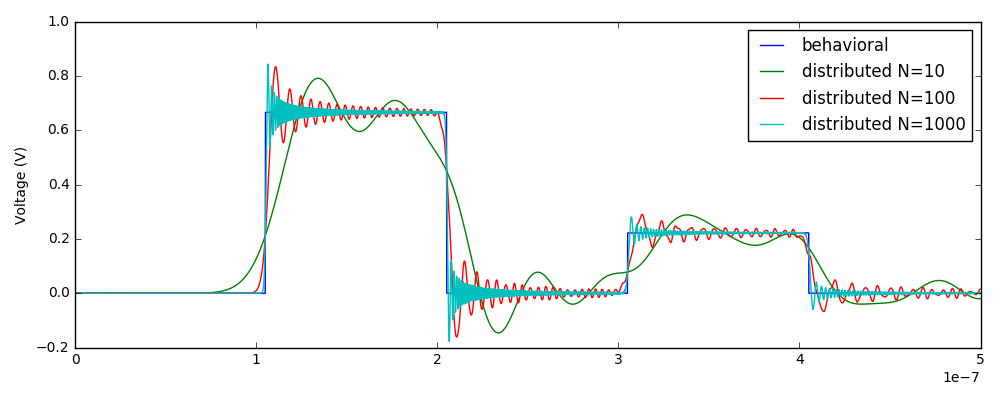
\includegraphics[width=0.3\textwidth]{src/2/figures/tline_comparison.pdf}
  \caption{Lumped versus two-port models comparison in simulation}
  \label{fig:lines-simulations}
\end{figure}

Le modèle comportemental surpasse le modèle distribué, autant en précision que temps de simulation.
Il reproduit parfaitement le temps de montée avec toutes les charges (Fig. \ref{fig:lines-simulations}).
Il est plus rapide à simuler de plusieurs ordres de grandeurs par rapport au modèle distribué.

La modélisation d'autres éléments importants tels que les composants passifs et les protections ESD est détaillé dans le document complet.

% Illustrate the method with a practical case
Pour illustrer l'application de la méthode de modélisation, elle est appliquée sur un banc TLP du laboratoire de NXP Toulouse.
C'est un bon cas d'étude afin d'utiliser la méthode, car ce banc est très largement utilisé pour l'investigation.
Pour démontrer sa précision, le modèle est vérifié par comparaison avec de multiples mesures, sous différentes charges et amplitudes.

\begin{figure}[!h]
  \centering
  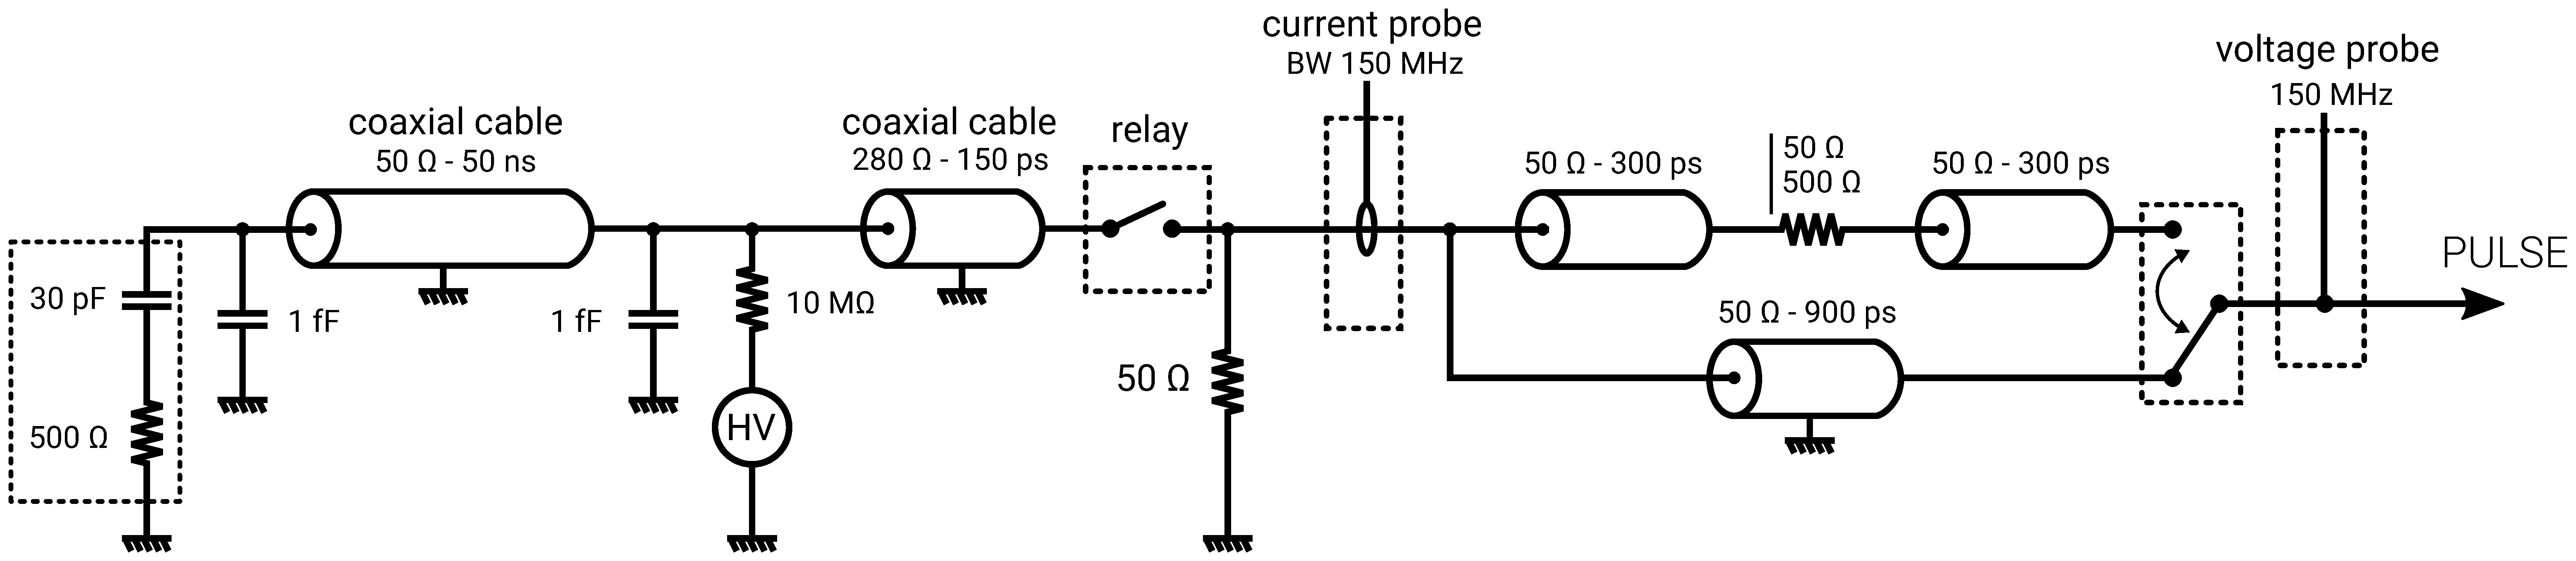
\includegraphics[width=\textwidth]{src/2/figures/complete_nxp_tlp_model.pdf}
  \caption{Complete model of NXP laboratory's TLP generator}
  \label{fig:complete-tlp-model}
\end{figure}

% Explain how the model, how it was constructed
Le modèle complet de TLP est donné en Fig. \ref{fig:complete-tlp-model}.
Il reproduit l'architecture du TLP du laboratoire en utilisant des modèles de la librairie pour chaque élément.
% Detail a first comparison with 25 ohms
Une première validation avec une mesure est donnée en Fig. \ref{fig:comparison-tlp-load}.
Avec une charge de 25\textOmega{} et une tension de charge de 500V, 4.5A et 125mV sont relevés sur le second plateau.
Le rapport de ces deux valeurs corresponds bien à 25\textOmega{} comme attendu.
Jusqu'à 220 ns, les deux courbes se ressemblent fortement.
Après, des différences apparaissent à cause des ondes réfléchies, qui entrainent une accumulation d'erreurs.
La plupart des simulations ESD restent intéressantes pendant la partie principale de la décharge jusqu'à 120ns et ces erreurs sont donc négligeables.

\begin{figure}[!h]
  \centering
  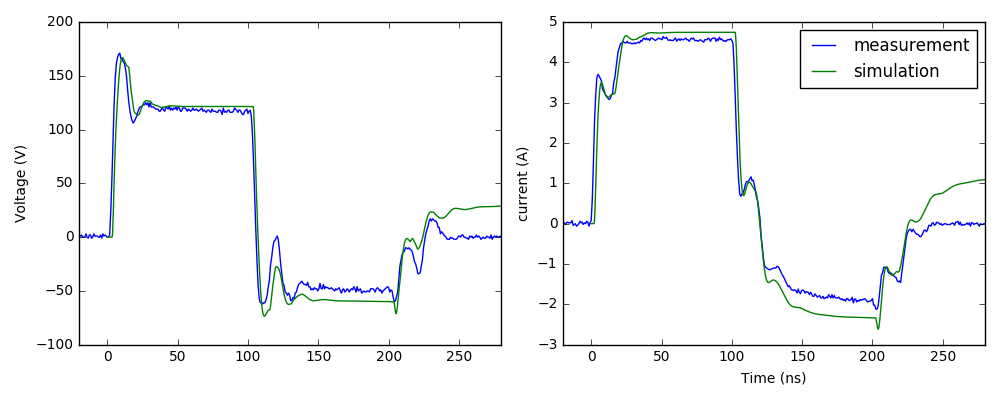
\includegraphics[width=\textwidth]{src/2/figures/tlp_comparison_R25_500V.png}
  \caption{Voltage and current waveforms comparison - 500 V charging voltage on 25\textOmega{}}
  \label{fig:comparison-tlp-load}
\end{figure}

% More validations in Annex
Les autres validations sont données dans le document complet, et présentent des niveaux de corrélations aussi proches.
Le modèle fonctionne correctement et reproduit les mesures, prouvant sa validité.

\section{Dévelopement d'un générateur TLP modifié}

%TODO: Simplifier
% TLP is a great tool for esd analysis
A travers cette étude et de manière générale, le TLP est utilisé très largement comme outil de characterization et de test.
Il est capable de générer des impulsions très bien controllées et reproductibles.
Néanmoins, il ne reproduit pas les formes d'ondes ESD rencontrés dans la réalité.
C'est pourquoi l'utilisation des pistolets ESD reste obligatoire pour la qualification de produits.
La forme d'onde la plus répandue est celle définie dans la spécification HMM \cite{hmm} et les standards IEC 61000-4-2 \cite{iec61000-4-2} et ISO 10605 standard \cite{iso10605}.
Ensemble, ils couvrent une très large plage d'applications, dans les domaines grand-public, automobile et industriel.
Pour combiner les avantages d'un TLP avec ceux d'une décharge HMM, un générateur TLP peut être modifié pour produire cette impulsion HMM.
Cette approche a été explorée par le passé par E. Grund \cite{iec61000-tlp} et Y. Cao \cite{tlp-based-hmm}.
Néanmoins, leurs techniques présentent quelques inconvénients tels que une tendance large à créer des oscillations, comme démontré dans le document complet.

Le générateur proposé ici est dénommé TLP-HMM.
Le TLP-HMM requiert deux modules additionnels à connecter à chaque extrémité d'un TLP standard 100ns.
Ils sont nommés \textit{absorber} et \textit{shaping filter} (Fig. \ref{fig:tlp_hmm_architecture}).
Le principe du TLP-HMM est de rerouter une portion du courant incident dans la masse, de manière à ce que le courant restant prenne la forme de l'onde HMM.

\begin{figure}[!h]
  \centering
  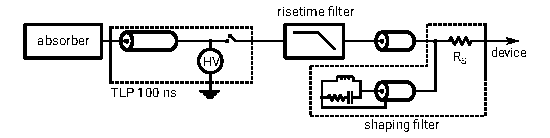
\includegraphics[width=0.9\textwidth]{src/5/figures/beges_tlp_hmm.pdf}
  \caption{TLP-HMM architecture}
  \label{fig:tlp_hmm_architecture}
\end{figure}

% Role of the shaping filter
Le shaping filter (Fig. \ref{fig:shaping_filter_example}) dévie le courant nécessaire pour former l'onde.
Il est composé de cinq éléments, un réseau RLC, un petit câble coaxial de délai \textDelta{}t, et une résistance d'injection.

\begin{figure}[!h]
  \centering
  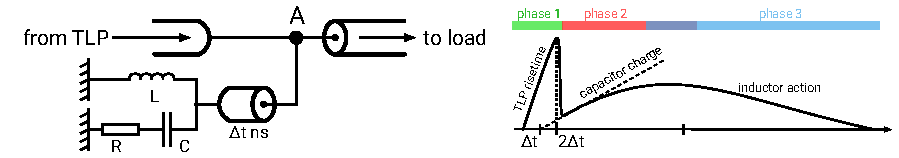
\includegraphics[width=0.98\textwidth]{src/5/figures/example_tlp_hmm.pdf}
  \caption{Shaping filter architecture and operation}
  \label{fig:shaping_filter_example}
\end{figure}

% Behavior of the filter - C
Une impulsion TLP rectangulaire est injectée sur la ligne principale (Fig. \ref{fig:shaping_filter_example}).
Elle atteint le point A à $t=0$ et la tension monte.
La capacité ne voit l'impulsion a $t=\Delta t$, et ne se charge que à partir de ce moment.
En retour, la charge est visible sur la ligne principale seulement à $t=2\Delta t$.
A cet instant, le potentiel chute sur la ligne principale, car la capacité devient visible et tire tout le courant.
Le premier pic de l'impulsion est ainsi créé, avec une durée d'environ $2\Delta t$.

% Behavior of L
Pendant que la capacité continue de se charger, l'inductance connectée en parallèle commence à absorber du courant à son tour.
A un moment donné, elle absorbe suffisamment de courant pour contrecarrer la charge de la capacité, et la tension commence à redescendre.
La décharge se poursuit lentement jusqu'à retourner à une tension nulle.
Le résultat de toutes ces actions est la création de la forme d'onde complète du HMM.

% Introduce the design
Le schéma exact du shaping filter est donné Fig. \ref{fig:shaping_filter_schematic}.
Le capacitance totale est distribuée pour réduire l'inductance parasite.
Les inductances sont également distribuées pour augmenter la capacité en courant.

\begin{figure}[!h]
  \centering
  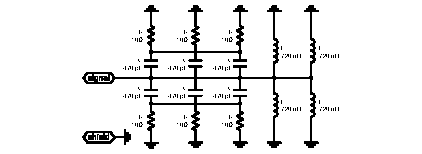
\includegraphics[width=0.9\textwidth]{src/5/figures/shaping_filter_schematic.pdf}
  \caption{shaping-filter schematic}
  \label{fig:shaping_filter_schematic}
\end{figure}

A la fin de la décharge, l'inductance continue d'absorber un courant important.
Si rien n'est fait, le potentiel au point pourrait être tiré négativement.
Pour empêcher cela, l'absorbeur lisse le front descendant de l'impulsion TLP sur une centaine de nanosecondes.
En ramenant doucement le courant à zéro, l'inductance s'arrête lentement d'absorber du courant et la tension reste nulle sans devenir négative.
La schématique de l'absorbeur est donnée Fig. \ref{fig:absorber_schematic}

\begin{figure}[!h]
  \centering
  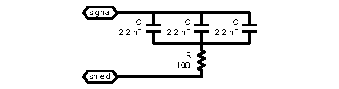
\includegraphics[width=0.7\textwidth]{src/5/figures/absorber_schematic.pdf}
  \caption{absorber schematic}
  \label{fig:absorber_schematic}
\end{figure}

Les courbes simulées et mesurées sur un prototype sont données Fig. \ref{fig:tlp_hmm_waveforms}.
Les courants mesurés à 30ns et 60ns sont dans la marge de tolérance de 30\% des standards, et elle est donc valide.

\begin{figure}[!h]
  \centering
  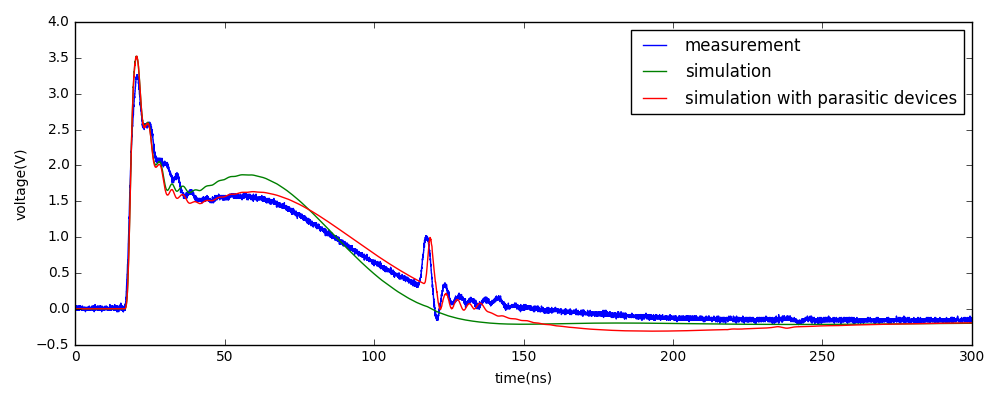
\includegraphics[width=0.95\textwidth]{src/5/figures/tlp_hmm_waveforms.png}
  \caption{Measurement versus simulation of a 250V TLP-HMM (equivalent 1kV HMM) on 2\textOmega{}}
  \label{fig:tlp_hmm_waveforms}
\end{figure}

% Analyse the curve
Globalement, la simulation et la mesure corrèlent bien.
Il y a des différences mineures, notamment entre 40ns and 150ns.
Elles sont dues à des éléments parasites non pris en compte durant les simulations, et des corrections sont à apporter au prototype.
L'analyse de ces éléments est fournie dans le document complet.

% Conclusion regarding TLP-HMM
Une nouvelle méthode pour générer des impulsions HMM avec un générateur TLP a été présentée.
Ce TLP-HMM fonctionne correctement, passe les conditions des standards avec succès et s'avère robuste contre les oscillations et perturbations externes.
Le prototype permet de valider le concept.
Le design doit être amélioré pour éliminer des éléments parasites.
Une tension de charge plus élévée doit aussi être disponible pour augmenter la capacité en courant du générateur actuellement limitée à 4A.

\section{Méthode de traitement de capteurs de courant on-chip}

%TODO next
% Introduction
La méthode de scan champ-proche a été présentée précédemment dans le chapitre 1.
Avec cette méthode il est possible de mesurer des cartographies de champ électrique ou magnétique.
Cela permet de localiser des sources de bruit haute-fréquence par exemple.
Il est aussi très intéressant de tenter de traiter les cartes de champs pour retrouver les valeurs de tension et courant à travers les sources d'émission.
Dans ce chapitre deux méthode de reconstruction sont évaluées, la première est purement temporelle et la seconde fréquentielle.
Le capteur de champ proche sur silicium présenté dans le chapître 3 est utilisé pour obtenir les mesures.

% What is the output voltage that is measured
La méthode temporelle consiste simplement à intégrer le signal mesuré en y appliquant des facteurs correctifs.
Il est montré dans \cite{near-field-scan} que cette approche est valide.
it is possible to express I\textsubscript{TLP} as a function of the measured sensor voltage V\textsubscript{sensor}.
Ici, l'étude se focalise sur le traitement d'une mesure magnétique pour retrouver un courant dans une piste en métal.
L'équation \ref{eq:nfs-rel2} donne la relation entre le courant dans la piste mesurée I\testsubscript{TLP} et la tension mesurée sur le capteur V\textsubscript{sensor}.

\begin{equation}
I_{TLP}(t) = \frac{1}{G}\int V_{sensor}(t) \mathrm{d}t + A
\label{eq:nfs-rel2}
\end{equation}

% How to determine 1/G and A
L'offset $A$ et le gain $1/G$ sont dus à l'intégration, et sont déterminés expérimentalement.
Le schéma de la méthode de mesure est donnée Fig. \ref{fig:calibration-sensor}.
Une impulsion rectangulaire de 100ns et 1V est injectée entre S1 et S2.
La tension V\textsubscript{sensor} est mesurée avec un oscilloscope 2GHz entre C1 et C2.

\begin{figure}[!h]
  \centering
  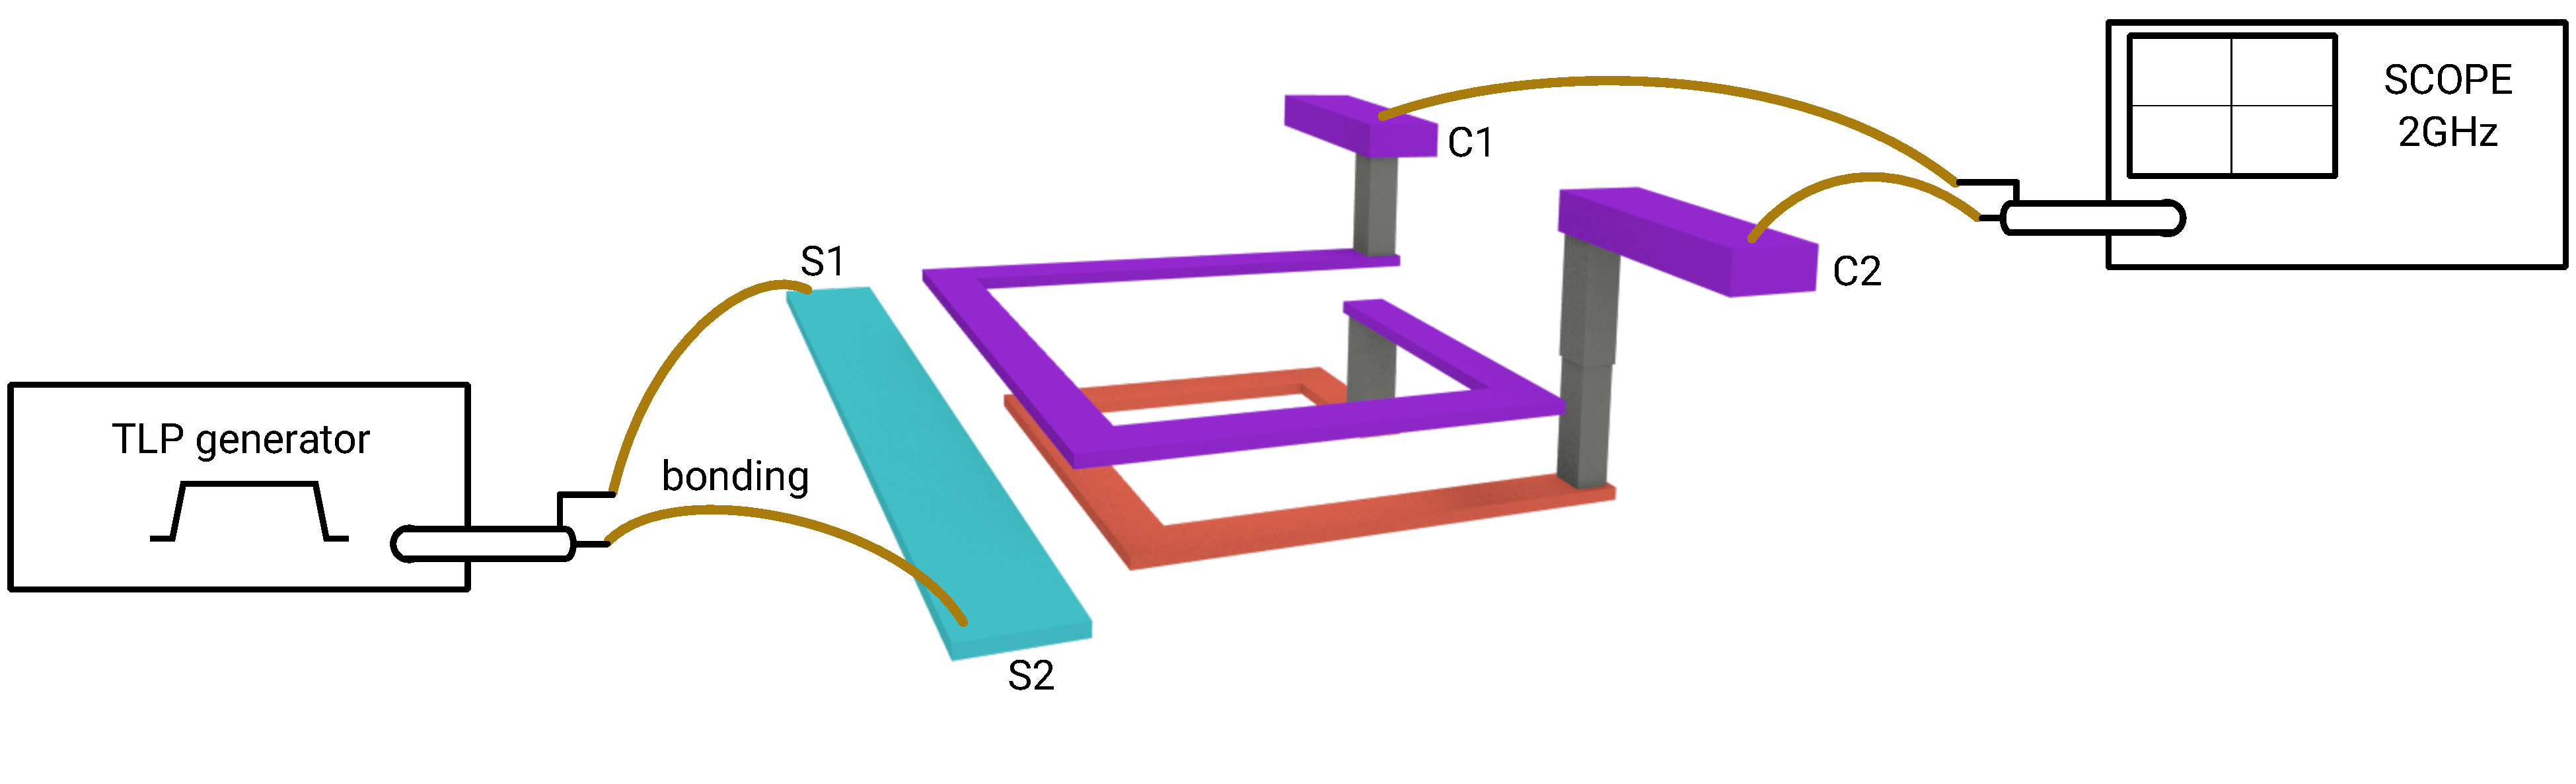
\includegraphics[width=0.9\textwidth]{src/3/figures/sensor_measurement_setup.pdf}
  \caption{Calibration sensor setup for time-domain method}
  \label{fig:calibration-sensor}
\end{figure}

% Explain the measurements
I\textsubscript{TLP} et V\textsubscript{sensor} sont mesurées et fournies Fig. \ref{fig:measurement-nfs}.
Ces courbes permettent d'estimer $1/G = 8.10^8$ et $A = -V_{TLP}(t = 0)$.

\begin{figure}[!h]
  \centering
  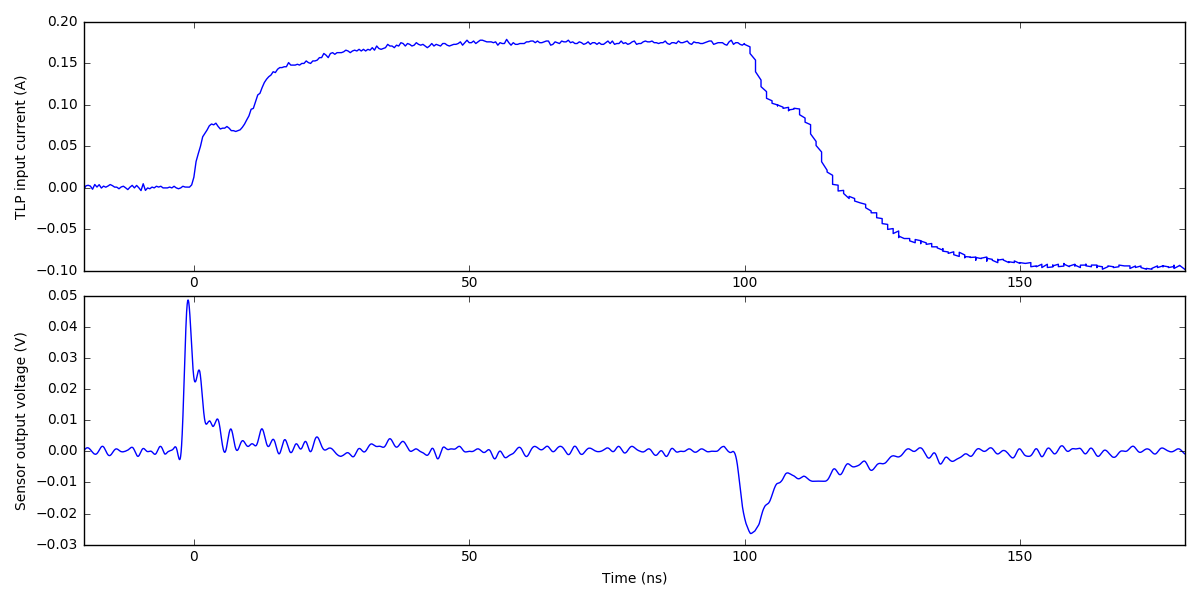
\includegraphics[width=0.95\textwidth]{src/3/figures/measured_waveform.png}
  \caption{Measured voltage waveform}
  \label{fig:measurement-nfs}
\end{figure}

% Intro & Characterization
La méthode fréquentielle utilise une mesure paramètre-S du capteur pour traiter V\textsubscript{sensor}.
Le montage de calibration est donné Fig. \ref{fig:calibration-sensor-rf}.

\begin{figure}[!h]
  \centering
  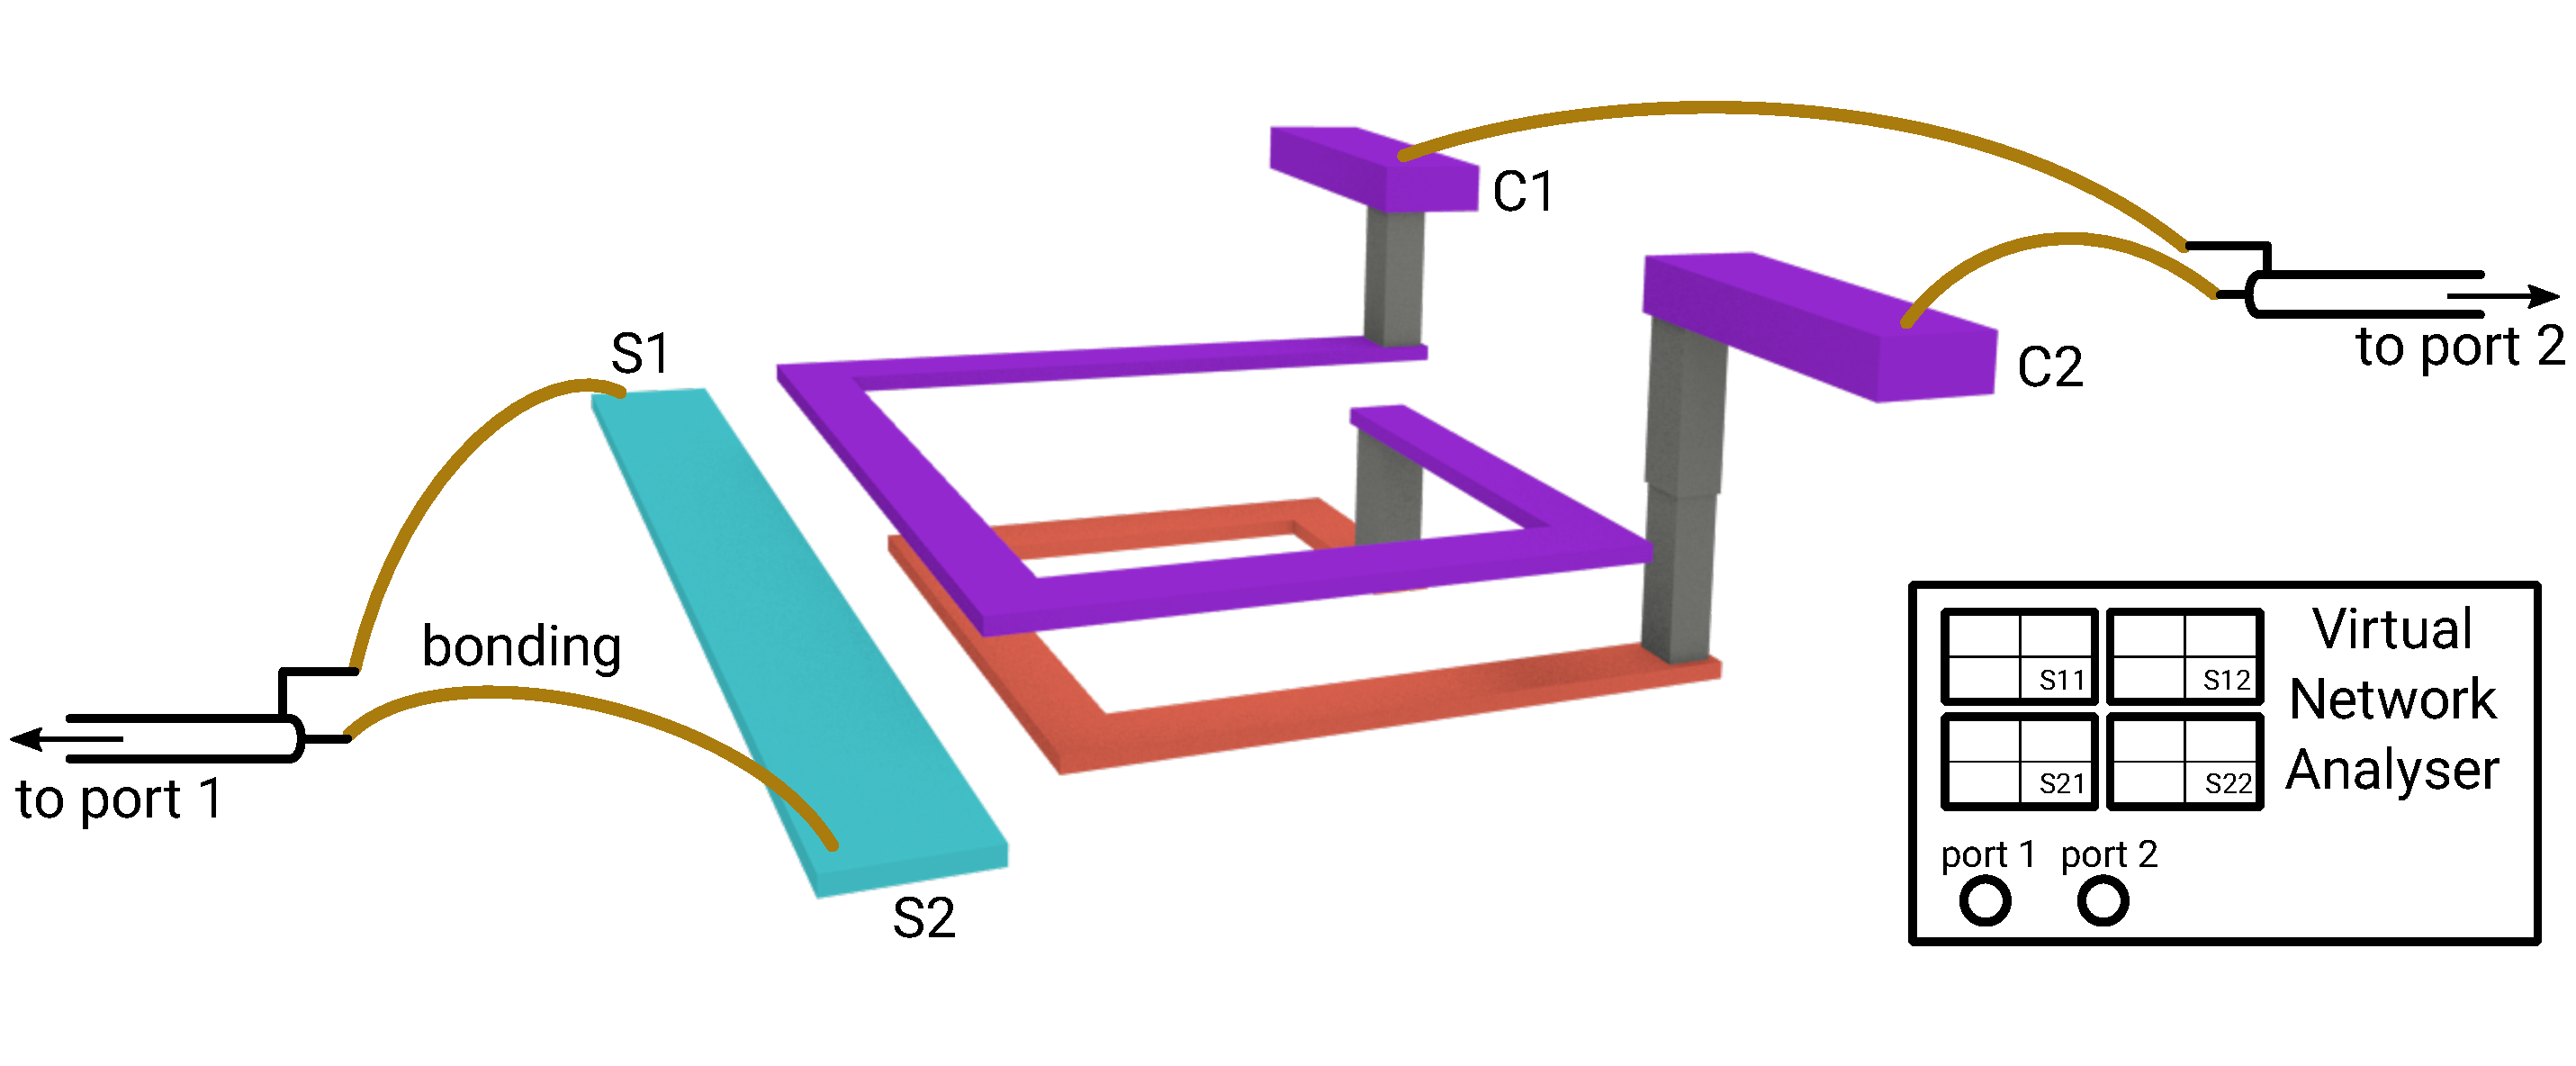
\includegraphics[width=0.9\textwidth]{src/3/figures/sensor_measurement_setup_rf.pdf}
  \caption{Calibration sensor setup for time-domain method}
  \label{fig:calibration-sensor-rf}
\end{figure}

% Detail characterization
La réponse du capteur en puissance transmise S21 est donné Fig. \ref{fig:sensor-response}.
Elle comprend une mesure du gain et du décalage de phase induits par le capteur.

\begin{figure}[!h]
  \centering
  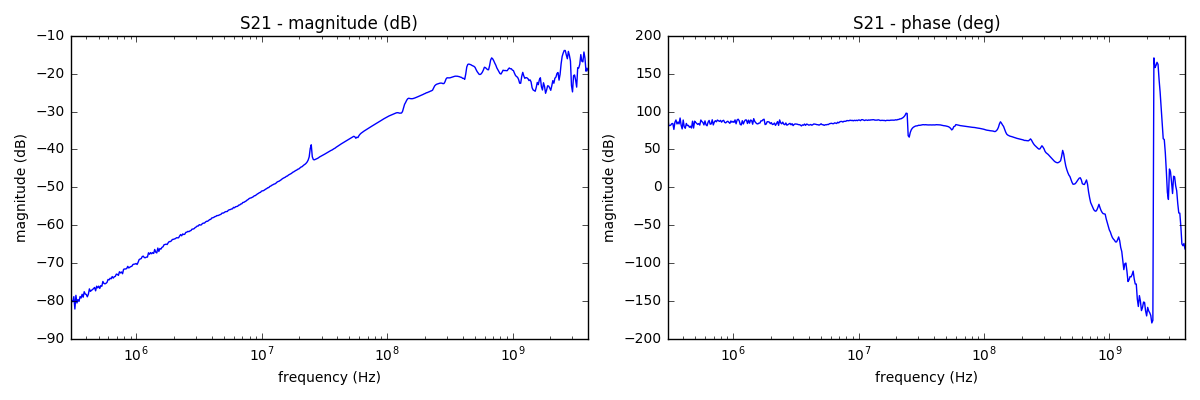
\includegraphics[width=0.9\textwidth]{src/3/figures/s21_freq_response.png}
  \caption{Sensor frequency response - complex S21 (magnitude and phase)}
  \label{fig:s21-response-complex}
\end{figure}

% The algorithm
L'algorithme de traitement est donné Fig. \ref{fig:postprocess-nfs-pipeline}.
La mesure temporelle est passée dans le domaine fréquentiel avec une FFT.
Diverses opérations de conversion pour passer en nombres complexes sont requises.
Une interpolation est nécessaire pour que les deux tableaux de nombres complexes partagent les mêmes valeurs sur l'axe des abscisses.
Ensuite, la mesure est compensée par la calibration en divisant simplement la première par la seconde.
Ceci permet de tenir compte pour chaque fréquence de la réponse du capteur.
Finalement, une FFT inverse permet de ramener la mesure compensée dans le domaine temporel.

\begin{figure}[!h]
  \centering
  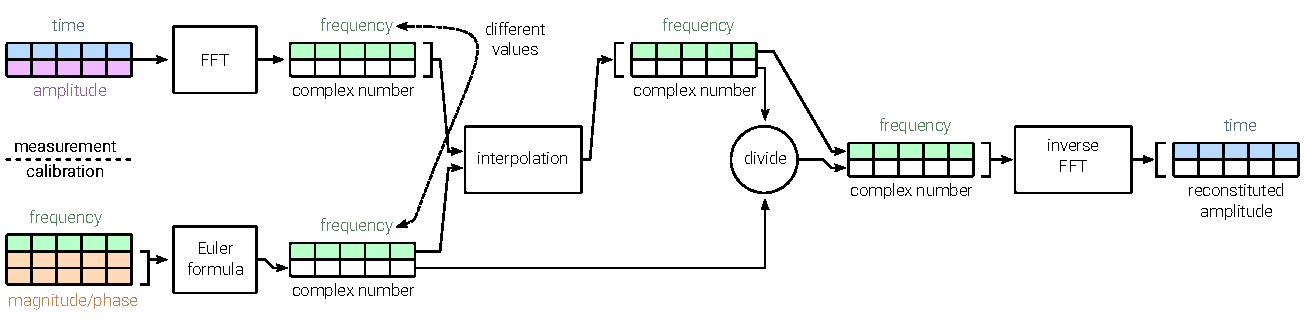
\includegraphics[width=\textwidth]{src/3/figures/frequency_post_process_flow.pdf}
  \caption{Post-processing pipeline}
  \label{fig:postprocess-nfs-pipeline}
\end{figure}

Une comparaison de la courbe originale, de la méthode temporelle, et de la méthode fréquentielle sont fournies Fig. \ref{fig:freq-domain-reconstructed}.
Globalement, les résultats sont similaires en terme de précision.
La méthode fréquentielle semble avoir une plus large dynamique.
Des erreurs sont présentes pour chacune après l'impulsion.
De multiples améliorations sont possibles, telles que augmenter le nombre de points de mesures pour obtenir une meilleure FFT et utiliser une meilleure méthode d'interpolation.

\begin{figure}[!h]
  \centering
  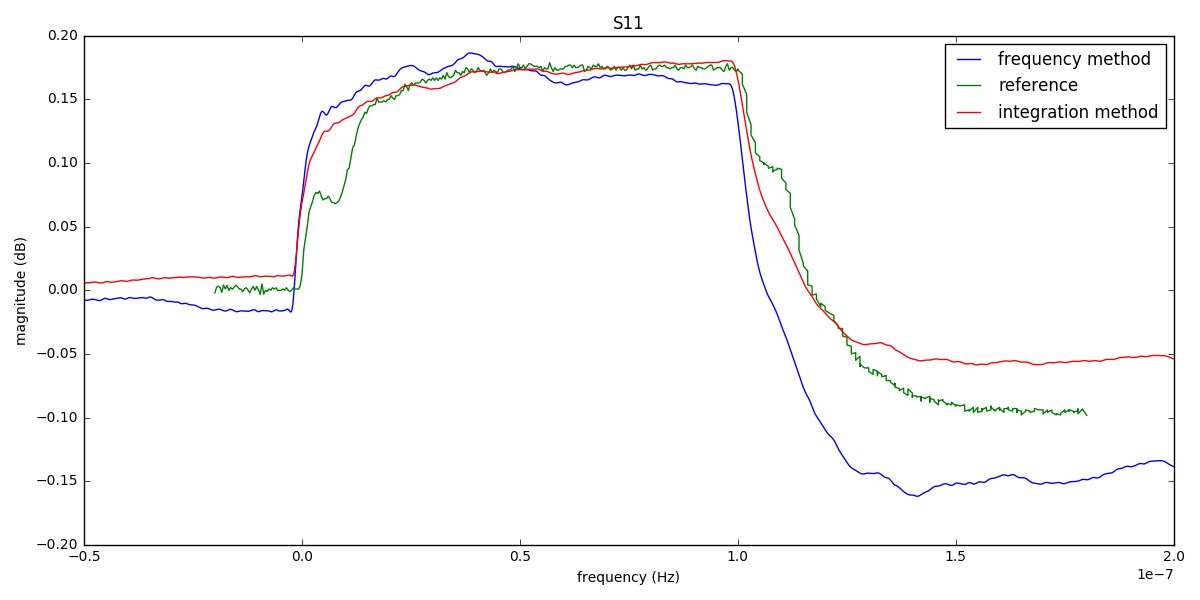
\includegraphics[width=0.9\textwidth]{src/3/figures/final_comparison_reconstructions.png}
  \caption{Reference current waveform versus frequency-domain and time-domain reconstructions}
  \label{fig:freq-domain-reconstructed}
\end{figure}
